% Information Sciences submission (roadmap M11, #130). Separate from the TFG manuscript doc/main3.tex.
% Plan: docs/publication/information_sciences.md. Red [pending: ...] marks are items still open.
% Supplementary material: supplementary.tex. Every number comes from generated/ (scripts/_emit_infsci_tables.py).
% Build from doc/infsci with: latexmk -pdf main.tex
\documentclass[preprint,review,12pt]{elsarticle}
\usepackage[T1]{fontenc}
\usepackage[utf8]{inputenc}
\usepackage{lmodern}
\usepackage{amsmath}
\usepackage{amsfonts}
\usepackage{amssymb}
\usepackage{amsthm}
\usepackage{graphicx}
\usepackage{float}
\usepackage{placeins}
\usepackage{xr}
\externaldocument[S-]{supplementary}
\usepackage{booktabs}
\usepackage{array}
\usepackage{xurl}
\usepackage{xcolor}
\usepackage{tikz}
\usepackage{microtype}
\usetikzlibrary{positioning,arrows.meta}
\graphicspath{{../images/}}
\newcolumntype{L}[1]{>{\raggedright\arraybackslash}p{#1}}
\newtheorem{proposition}{Proposition}
\newtheorem{remark}{Remark}
\newcommand{\pending}[1]{\textcolor{red}{[pending: #1]}}
\setlength{\emergencystretch}{2em}
% generated by scripts/_emit_infsci_tables.py; do not edit
\newcommand{\floatMaxRP}{1.4e-13}
\newcommand{\floatMaxGASF}{5.6e-17}
\newcommand{\floatMaxGADF}{8.4e-17}
\newcommand{\floatMaxXIRP}{2.8e-16}
\newcommand{\floatBlocksExactRP}{19}
\newcommand{\rpEightMin}{0.0009}
\newcommand{\rpEightMax}{0.0022}
\newcommand{\rpEightSwarmMin}{0.012}
\newcommand{\rpEightSwarmMax}{0.017}
\newcommand{\benchSeries}{54\,336}
\newcommand{\benchBlocks}{20}
\newcommand{\macroDiffRPHIRATA}{0.185}
\newcommand{\macroDiffRPHIRATASIGNED}{0.084}
\newcommand{\macroDiffRPUNSIGNED}{0.122}
\newcommand{\macroDiffMTF}{0.311}
\newcommand{\binaryOracleMin}{0.03}
\newcommand{\binaryOracleMax}{0.17}
\newcommand{\condGoodSeries}{47\,949}
\newcommand{\condGoodBad}{0}
\newcommand{\condWorstRate}{85}
\newcommand{\speedupMid}{2.9}
\newcommand{\speedupLong}{5.2}
\newcommand{\clsCombos}{84}
\newcommand{\clsCombosEq}{66}
\newcommand{\clsWindows}{90\,937}
\newcommand{\escWindows}{18\,000}
\newcommand{\escCombos}{36}
\newcommand{\robHighRP}{0.041}
\newcommand{\robHighGASF}{0.064}
\newcommand{\robHighGADF}{0.064}
\newcommand{\robHighXIRP}{0.011}
\newcommand{\robDatasetsRPBetter}{6}
\newcommand{\robDatasets}{7}
\newcommand{\robLossyShift}{0.019}
\newcommand{\srRPFivehundred}{0.0076}
\newcommand{\srColFivehundred}{0.08}
\newcommand{\srShareFivehundred}{67}
\newcommand{\srRPTwofifty}{0.0041}
\newcommand{\srColTwofifty}{0.16}
\newcommand{\srShareTwofifty}{23}
\newcommand{\srRPHundred}{0.0015}
\newcommand{\srColHundred}{0.37}
\newcommand{\srShareHundred}{0}
\newcommand{\srRPFifty}{0.0009}
\newcommand{\srColFifty}{0.61}
\newcommand{\srShareFifty}{0}
\newcommand{\srGafMin}{0.0018}
\newcommand{\srGafMax}{0.0032}
\newcommand{\srNativeRP}{0.0015}
\newcommand{\srResampledRP}{0.0015}


\journal{Information Sciences}

\begin{document}

\begin{frontmatter}

\title{How Much of a Time Series Survives Its Image? A Cross-Domain Comparative Analysis of the Reconstruction Capacity of Image-Based Representations}

\author[mydass]{Adriano García-Giralda Milena}
\author[cls]{Francisco García Moreno}
\author[alg]{José Antonio Jiménez Madrid}
\author[cls]{María Bermúdez Edo}

\affiliation[mydass]{organization={MYDASS Research Group, University of Granada}, country={Spain}}
\affiliation[cls]{organization={Department of Computer Languages and Systems, University of Granada}, country={Spain}}
\affiliation[alg]{organization={Department of Algebra, University of Granada}, country={Spain}}

\begin{abstract}
% <= 200 words.
Image-based representations have been widely studied for time-series classification, while recent work has also demonstrated their use for image-based synthesis and imputation. Yet successful generation does not establish what different encodings preserve or whether their images can be reliably decoded into signals. We investigate this question for binary, unsigned and signed recurrence plots (RP), Gramian angular summation and difference fields (GASF/GADF), and Markov transition fields (MTF), using the invertible-by-design XIRP as a reference. Alongside established inverses, we introduce an image-only geometric decoder for signed RP, a restricted-range GADF decoder, and an approximate MTF reconstruction procedure.

Across seven datasets from six domains, we evaluate temporal and spectral fidelity, robustness, computational cost and downstream classification utility, distinguishing encoding losses from 8-bit storage effects. Under stated conditions, signed RP, GASF, restricted-range GADF and XIRP allow numerically exact reconstruction from floating-point matrices; storage introduces additional error, particularly for ill-conditioned RP states. Unsigned RP retains a global-reflection ambiguity, whereas binary RP and MTF are intrinsically many-to-one.

These findings establish a reproducible comparison of reconstruction capabilities and limitations, informing future research on generating time series through image-domain models.
\end{abstract}

\begin{keyword}
% 1-7 keywords
Time-series imaging \sep Reconstruction \sep Recurrence plots \sep Gramian angular fields \sep Markov transition fields \sep Invertibility \sep Comparative analysis
\end{keyword}

\end{frontmatter}

% ============================================================================================
\section{Introduction}\label{sec:introduction}

Image-based representations transform time series into structured matrices that can be processed using techniques originally developed for images. Recurrence plots (RP), Gramian angular fields (GAF) and Markov transition fields (MTF) have been widely explored for time-series classification and related tasks~\cite{wang2015encoding,wang2015encoding2,eckmann1987recurrence,marwan2007recurrence}. In classification, a representation need only preserve information relevant to the target task; reconstructing the original waveform is not necessarily required. However, applications that aim to recover or synthesise temporal signals introduce a different requirement: the encoded images must retain sufficient information to reconstruct meaningful time series.

Recent research has demonstrated the feasibility of exploiting image-based generative models for temporal data. Huang et al.~\cite{huang2023tsdigan} used Gramian angular representations with generative adversarial networks for traffic-data imputation. More recently, Hellermann and Lessmann~\cite{hellermann2026imagegan} introduced the extended intertemporal return plot (XIRP), an invertible-by-design representation for time-series generation through image-based GANs, with competitive predictive utility against specialised generative approaches. Successful synthesis using particular representations does not establish the reconstruction capabilities of other encodings, nor the conditions under which their information can be recovered.

Reconstructing an image produced by a known encoder does not guarantee that an arbitrary image generated by a learned model represents a valid time series, so characterising reconstruction is a necessary preliminary investigation, not a demonstration of generative performance.

In this work, we establish a common framework for evaluating the reconstruction capabilities of image-based representations built from relationships between temporal samples or states. We examine binary, continuous unsigned and signed RP; Gramian angular summation and difference fields (GASF/GADF); and MTF. XIRP is included as an invertible-by-design reference developed for generative applications. All of them are pairwise relational matrices, whose entry $(i,j)$ relates two instants or states. Time-frequency and time-scale representations, such as spectrograms and scalograms, are outside the scope of this study, as are transforms that reshape or fold the samples themselves into a grid, such as the delay embedding used for diffusion-based generation by Naiman et al.~\cite{naiman2024imagentime}, which are invertible by construction.

All methods are evaluated under a common 8-bit image-storage protocol, decoding from the stored image alone (Figure~\ref{fig:workflow}); for recurrence plots, comparisons with the approaches of Hirata et al.~\cite{hirata2008reproduction} and Sipers et al.~\cite{sipers2017robust} separate the encoding from the decoder.

\begin{figure}[!t]
\centering
\resizebox{\textwidth}{!}{%
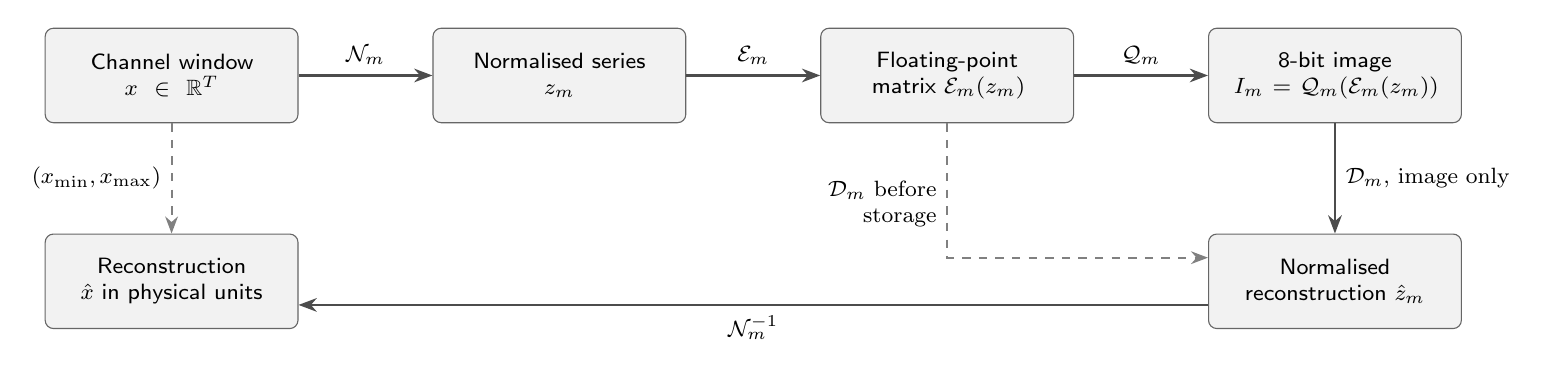
\begin{tikzpicture}[font=\sffamily\footnotesize\linespread{1}\selectfont, node distance=14mm and 17mm,
  box/.style={rectangle, rounded corners=3pt, draw=black!60, fill=black!5,
    align=center, minimum height=12mm, text width=3cm, inner sep=3pt},
  arrow/.style={->, draw=black!70, line width=0.8pt, >=Stealth},
  side/.style={->, draw=black!50, dashed, line width=0.7pt, >=Stealth},
  lab/.style={font=\footnotesize\linespread{1}\selectfont, fill=white, inner sep=1.5pt}]
\node[box] (input) {Channel window\\$x\in\mathbb{R}^{T}$};
\node[box, right=of input] (calib) {Normalised series\\$z_m$};
\node[box, right=of calib] (float) {Floating-point\\matrix $\mathcal E_m(z_m)$};
\node[box, right=of float] (image) {8-bit image\\$I_m=\mathcal Q_m(\mathcal E_m(z_m))$};
\node[box, below=of image] (zhat) {Normalised\\reconstruction $\hat z_m$};
\node[box, below=of input] (xhat) {Reconstruction\\$\hat x$ in physical units};
\draw[arrow] (input) -- node[lab, above=2pt] {$\mathcal N_m$} (calib);
\draw[arrow] (calib) -- node[lab, above=2pt] {$\mathcal E_m$} (float);
\draw[arrow] (float) -- node[lab, above=2pt] {$\mathcal Q_m$} (image);
\draw[arrow] (image) -- node[lab, right=2pt] {$\mathcal D_m$, image only} (zhat);
\draw[side] (float.south) |- node[lab, pos=0.3, left=2pt, align=right] {$\mathcal D_m$ before\\storage} ([yshift=3mm]zhat.west);
\draw[arrow] ([yshift=-3mm]zhat.west) -- node[lab, below=2pt] {$\mathcal N_m^{-1}$} ([yshift=-3mm]zhat.west -| xhat.east);
\draw[side] (input) -- node[lab, left=2pt] {$(x_{\min},x_{\max})$} (xhat);
\end{tikzpicture}}
\caption{Controlled reconstruction protocol for one channel $x$ and representation $m$. The channel is calibrated by $\mathcal N_m$, encoded by $\mathcal E_m$ and stored as an 8-bit image by $\mathcal Q_m$. The decoder $\mathcal D_m$ recovers a normalised trajectory $\hat z_m$ from the image alone; the channel's minimum and maximum in the window are used only by $\mathcal N_m^{-1}$ to return to physical units. Decoding the floating-point matrix (dashed) isolates reconstruction error from storage error.}\label{fig:workflow}
\end{figure}

We address four research questions:
\begin{itemize}
\item \emph{RQ1 --- Recoverability.} What information can be recovered from each representation, in both the time and frequency domains, and how much is lost through encoding and 8-bit storage?
\item \emph{RQ2 --- Reconstruction methods.} Under which conditions are the proposed decoders exact, and how do the encoding and decoding stages separately influence recurrence-plot reconstruction?
\item \emph{RQ3 --- Robustness and stability.} How do image perturbations, quantisation and signal characteristics, including sampling rate and state-space conditioning, affect reconstruction fidelity?
\item \emph{RQ4 --- Computational and downstream utility.} What are the computational costs of reconstruction, and to what extent do reconstructed signals preserve the performance of classifiers trained on original data?
\end{itemize}

The main contributions of this study are:
\begin{itemize}
\item \emph{A reproducible reconstruction benchmark.} We systematically evaluate temporal image representations across seven public datasets from six domains, using a common protocol covering temporal and spectral fidelity, robustness, computational cost and downstream classification utility. This allows intrinsic representation losses to be distinguished from storage-related errors.
\item \emph{New reconstruction procedures and theoretical characterisation.} Our main methodological contribution is a geometric image-only decoder for signed RP, together with sufficient conditions for exact recovery. It is complemented by an anchored decoder for restricted-range GADF and an approximate reconstruction procedure for MTF, the latter as a control for an encoding that loses information. Controlled RP comparisons further separate the effects of directional information, distance preservation and decoder design.
\item \emph{An empirical foundation for image-based time-series generation.} We identify which representations admit reliable reconstruction, the ambiguities they retain and the conditions affecting stability, without assuming that reconstruction fidelity alone determines the quality of synthetic time series.
\end{itemize}

\section{Related work}\label{sec:related}

\paragraph{Temporal image encodings}
Recurrence plots (RP) visualise recurrences in an embedded state space, conventionally through a binary neighbourhood relation~\cite{eckmann1987recurrence,marwan2007recurrence}. Continuous RP variants preserve state distances; the modified signed RP of Lu and Tong additionally provides directional information~\cite{lu2019robust}. Wang and Oates introduced Gramian angular summation and difference fields (GASF/GADF) and Markov transition fields (MTF) as image representations for classification and imputation~\cite{wang2015encoding,wang2015encoding2}. Their subsequent use in activity recognition and anomaly detection illustrates the value of these encodings as predictive features~\cite{ahmad2021inertial,ma2024anomaly}. Predictive usefulness, however, does not establish whether the original waveform can be recovered.

\paragraph{Reconstruction from encoded images}
The inverse problem has been investigated most directly for RP. Hirata et al.\ reconstruct state-space geometry from binary recurrence information, using graph-based distances and multidimensional scaling~\cite{hirata2008reproduction,hirata2016chromosome}. Thiel et al.\ showed that, under certain conditions, a binary RP retains enough information to reconstruct the attractor up to its topology~\cite{thiel2004information}, and Hirata et al.\ later refined the reconstruction of a continuous series from a sparse RP coarse to fine, from Jaccard coefficients of neighbour sets, at a cost linear in its length~\cite{hirata2021fast}. For unthresholded RP, Sipers et al.\ establish identifiability conditions up to mean and global sign and develop a spectral reconstruction method, including experiments on disturbed and multilevel images~\cite{sipers2011unique,sipers2017robust}. These results concern unsigned recurrence information and therefore do not resolve orientation using the directional content of a signed RP. For GASF, the diagonal inverse on a nonnegative normalisation is already known and has supported image-based imputation~\cite{wang2015encoding,huamin2020reconstruction}. By contrast, GADF retains angular differences but not an immediately available absolute reference, and MTF quantisation discards within-state amplitudes.

\paragraph{Image-domain generation and the remaining question}
Image-based imputation~\cite{huang2023tsdigan} and generation~\cite{hellermann2026imagegan} need the reverse map from image to series. XIRP solves it by design, storing the normalised trajectory on its diagonal; for the other encodings it remains open what the image determines, how a decoder can use it, and how 8-bit storage and perturbations affect the result.

\section{Mathematical formulation}\label{sec:formulation}

\subsection{Reconstruction problem and information retained}

Let $x=(x_1,\ldots,x_T)$ denote a non-constant window of one signal channel. For representation $m$, the calibrated series $z_m=\mathcal N_m(x;x_{\min},x_{\max})$ lies in a predefined normalised domain, specific to each representation: $[0,1]$ for GASF, $[-0.7,0.7]$ for GADF and $[1,2]$ for XIRP, while MTF uses quantile states. The continuous RP images are unchanged by any increasing affine map of the series, because distances do not depend on a translation and the storage rule removes the scale (Section~\ref{sec:storage}); so is the binary RP, because its threshold is set in each window by a fixed recurrence rate rather than in physical units; we therefore compute them on the window as recorded, which gives the same stored image as $z_m=(x-x_{\min})/(x_{\max}-x_{\min})$. The RP decoders recover the trajectory up to a translation and a positive scale, which they fix by mapping its range onto $[0,1]$; this is $\hat z_m$. Only then does $\mathcal N_m^{-1}$ use the calibration, and the implementation composes these two affine maps into one. It is encoded as a matrix, stored as an 8-bit image, and decoded according to
\[
I_m=\mathcal Q_m\bigl(\mathcal E_m(z_m)\bigr),\qquad
\hat z_m=\mathcal D_m(I_m),\qquad
\hat x=\mathcal N_m^{-1}(\hat z_m;x_{\min},x_{\max}).
\]
Here $\mathcal Q_m$ is a predefined storage \emph{rule}, possibly with a per-image affine range. The term \emph{image-only} refers to $\hat z_m$: decoding never accesses the original window or window-specific side information. The pair $(x_{\min},x_{\max})$ is the minimum and maximum of the channel in that window. It is used only to express $\hat x$ in physical units and never to decode $\hat z_m$; a future image-based generator would have to supply it separately (Figure~\ref{fig:workflow}).

For readability, encoding formulas below use $x$ to denote the calibrated signal $z_m$. Three properties must be distinguished. \emph{Identifiability} concerns whether two admissible normalised signals can produce the same encoded matrix, possibly up to a specified symmetry. \emph{Decoder exactness} concerns whether $\mathcal D_m\circ\mathcal E_m$ recovers the original normalised signal under stated hypotheses, before storage. \emph{Stability} concerns how errors in the image, including quantisation, propagate to the decoded signal. A many-to-one encoder cannot admit a universally exact inverse, irrespective of decoder design. Conversely, a mathematically identifiable signal may still be reconstructed inaccurately from an 8-bit image if the inverse is poorly conditioned.

\subsection{Recurrence plots}\label{sec:rp_encodings}

For all RP variants we use adjacent two-sample states,
\[
s_i=(x_i,x_{i+1})\in\mathbb R^2,\qquad i=1,\ldots,T-1,
\]
that is, a two-dimensional delay embedding with unit delay~\cite{takens1981detecting}. The variants differ in how much information they retain about pairwise state displacements.

The \emph{binary RP} records neighbourhood membership,
$B_{ij}=\mathbb 1[\lVert s_i-s_j\rVert_2<\varepsilon]$, where we choose $\varepsilon$ in each window so that a fixed share of the off-diagonal pairs, the recurrence rate, is recurrent.
Thresholding discards the underlying distances, making the encoding many-to-one~\cite{eckmann1987recurrence,marwan2007recurrence}.
The \emph{continuous unsigned RP} stores
$D_{ij}=\lVert s_i-s_j\rVert_2$, scaled by $\max_{ij}D_{ij}$.
As a Euclidean distance matrix, $D$ determines the embedded states up to translation and an orthogonal transformation. In particular, reflecting all signal values leaves $D$ unchanged. Recovery up to global reflection therefore requires additional non-degeneracy assumptions; the unsigned image cannot determine the absolute orientation by itself~\cite{sipers2011unique}.

The \emph{signed RP} of Lu and Tong~\cite{lu2019robust} associates a directional label with each distance. With $v=(1,1)/\sqrt2$ and $\hat u_{ij}=(s_i-s_j)/\lVert s_i-s_j\rVert_2$ for nonzero displacements, its encoding is
\begin{equation}
R_{ij}=\sigma_{ij}\lVert s_i-s_j\rVert_2,\qquad
\sigma_{ij}=\begin{cases}
+1,&\lVert s_i-s_j\rVert_2=0\ \text{or}\ \hat u_{ij}\cdot v\ge\cos(\pi/4),\\
-1,&\text{otherwise}.
\end{cases}
\label{eq:signed_rp}
\end{equation}
Its magnitude recovers the unsigned matrix, $|R|=D$. Directional information can additionally distinguish a signal from its global reflection: a pair is \emph{sign-informative} when its displacement lies within $\pi/4$ of $v$ or $-v$, i.e.\ $|\hat u_{ij}\cdot v|\ge\cos(\pi/4)$, in which case $\sigma_{ij}=-\sigma_{ji}$; because the inequality in~\eqref{eq:signed_rp} is weak, this also holds on the boundary $|\hat u_{ij}\cdot v|=\cos(\pi/4)$. Other nonzero pairs receive the same negative sign in both directions. Thus the signed RP adds information that is absent from the distance matrix, but this alone does not guarantee unique reconstruction. Its per-window affine image storage retains the quantised zero level through the diagonal (Section~\ref{sec:storage}).

For exact-input recovery, three issues must be resolved: the embedded geometry must be recoverable from distances; consecutive embedded states must determine a consistent one-dimensional trajectory; and the signed information must distinguish the remaining reflection. Proposition~\ref{prop:rp} states sufficient conditions for each, for the geometric decoder of Section~\ref{sec:rp_decoder}. Let $\bar s$ be the mean state and $\sigma_1\ge\sigma_2\ge0$ the singular values of the centred state matrix $S-\mathbf 1\bar s^\top$, whose rows are $s_i-\bar s$.

\begin{proposition}[Signed RP on exact input]\label{prop:rp}
Assume that
\begin{enumerate}
\item[(a)] $\sigma_2>0$, i.e.\ the centred states span $\mathbb R^2$;
\item[(b)] there are no constants $\kappa$ and $(\alpha,\beta)\neq(0,0)$ such that either \emph{(R)} $x_i+x_{i+2}=\kappa$ for all $i=1,\ldots,T-2$, or \emph{(F)} $\alpha(x_{i+2}-x_i)=\beta x_{i+1}+\kappa$ for all $i=1,\ldots,T-2$;
\item[(c)] at least one pair of states is sign-informative.
\end{enumerate}
Then the decoder of Section~\ref{sec:rp_decoder}, applied to the floating-point signed RP, returns $x$ on the normalised domain. Without (c), $x$ and $-x$ have the same signed RP, so no image-only decoder can tell them apart. Under (a), condition (b) holds if and only if one of the matrices $H_\eta$ of step~3 has a simple zero eigenvalue and the other is positive definite, so it can be checked from the image; it holds, in particular, when the centred triples $(x_i,x_{i+1},x_{i+2})$, $i=1,\ldots,T-2$, have rank three.
\end{proposition}

\noindent\emph{Proof sketch.} Under (a), classical MDS recovers the states up to a translation and an orthogonal transformation~\cite{Torgerson1952}. Among those configurations, the overlap residual $b_i-a_{i+1}$ is constant only for the identity and its negative when (b) holds, i.e.\ for the states of $x$ and $-x$. Reflecting the series changes the sign of exactly the sign-informative entries, so the two signed RPs differ if and only if (c) holds, and the sign comparison of step~5, which re-encodes the assembled series of all four candidates, then selects $x$. The full proof is given in Supplementary Section~\ref{S-sec:s_proof}.

None of these conditions follows from the others. For the sinusoid at a quarter of the sampling rate, $x_i=\sin(\pi i/2+\phi)$, the states span the plane but (R) holds, every rotation satisfies the overlap, and the phases $\phi=0.2$ and $\phi=0.25$ give the same signed RP, so identifiability is lost altogether, not only up to sign. The series $x=(1,-1.05,1.10,-1.15,1.20,-1.25,1.30,-1.35)$ satisfies (a) and (b), but every displacement lies close to the anti-diagonal, so no pair is sign-informative and $x$ and $-x$ have the same signed RP. The conditions are sufficient, not necessary. All \hypSeries{} benchmark series satisfy (a)--(c) when checked directly (Supplementary Section~\ref{S-sec:s_hypotheses}), and the floating-point decoder recovered every one of them to numerical precision (Section~\ref{sec:results_fidelity}).

The proposition concerns exact input, not stability after storage. For exact input, the doubly centred Gram matrix used by classical MDS has nonzero eigenvalues $\sigma_1^2$ and $\sigma_2^2$, so the gap separating the recovered two-dimensional subspace from the remaining eigenvalues is $\sigma_2^2$. By the Davis--Kahan theorem, a perturbation of that matrix rotates the subspace by an amount bounded by the perturbation divided by this gap~\cite{davis1970rotation}. We therefore report the scale-free ratio $\sigma_2/\sigma_1$ as an empirical indicator of geometric conditioning, not as a bound on the reconstruction error: quantisation, the recovery of the zero level from the diagonal, the overlap orientation and the sign decision introduce further errors.

\subsection{Gramian angular fields}

GASF and GADF encode pairwise angular relations~\cite{wang2015encoding}. A normalised sample $\tilde x_i\in[-1,1]$ is mapped to $\phi_i=\arccos\tilde x_i$, giving
\[
G^{\mathrm S}_{ij}=\cos(\phi_i+\phi_j),\qquad
G^{\mathrm D}_{ij}=\sin(\phi_i-\phi_j).
\]
Their inverse properties differ substantially. For \emph{GASF}, the diagonal is $G^{\mathrm S}_{ii}=\cos(2\phi_i)$. It is ambiguous over $[-1,1]$ but injective when samples are normalised to $[0,1]$, as in our experiments; there $\tilde x_i=\cos\!\bigl(\tfrac12\arccos G^{\mathrm S}_{ii}\bigr)$. Thus GASF has a direct image-only inverse under the stated normalisation.

For \emph{GADF}, the diagonal is identically zero and only relative angular differences are available. Recovering the series requires both a unique branch of $\arcsin$ and an angular reference. With per-window normalisation to $[-\alpha,\alpha]$, the maximum angle separation is
\[
\max_{i,j}|\phi_i-\phi_j|=\pi-2\arccos\alpha
<\frac\pi2\qquad\text{if}\quad \alpha<\frac1{\sqrt2}.
\]
We use $\alpha=0.7$, so angular differences remain on the principal branch. Because every non-constant calibrated window reaches both endpoints, the global offset can then be fixed using the image itself (Section~\ref{sec:gadf_decoder}). This conditional inverse does not extend to arbitrary GADF normalisations: outside the restricted interval, branch ambiguities may remain.

\subsection{Markov transition fields}

MTF first assigns each sample to a quantile state $q_t\in\{1,\ldots,Q\}$ and estimates the transition probabilities $W_{pq}=P(q_{t+1}=q\mid q_t=p)$~\cite{wang2015encoding}. The image is then defined by $M_{ab}=W_{q_aq_b}$. It retains information about the temporal arrangement of discrete states but discards within-state amplitudes; moreover, numerical state ordering cannot generally be inferred uniquely from the image. Different waveforms can therefore yield the same MTF. In this setting reconstruction is necessarily approximate: the decoder selects a representative trajectory rather than recovering a uniquely determined original.

\subsection{Extended intertemporal return plot}

XIRP was proposed specifically for image-based time-series generation~\cite{hellermann2026imagegan}. For a strictly positive normalised series it combines intertemporal log returns with an explicit record of the sample values:
\[
R_{ij}=\begin{cases}
\log(x_i/x_j),&i\ne j,\\
x_i,&i=j.
\end{cases}
\]
The diagonal thus provides an exact inverse before storage, while every off-diagonal column supplies additional estimates through $x_i=x_j\exp(R_{ij})$. We map each channel to $[1,2]$ with the common calibration and include XIRP as an \emph{invertible-by-design reference}, not as another conventional classification encoding.

Table~\ref{tab:contract} summarises these recoverability properties; Figure~\ref{fig:encodings} displays the actual stored images for representative signal windows.

\begin{figure}[!htbp]
\centering
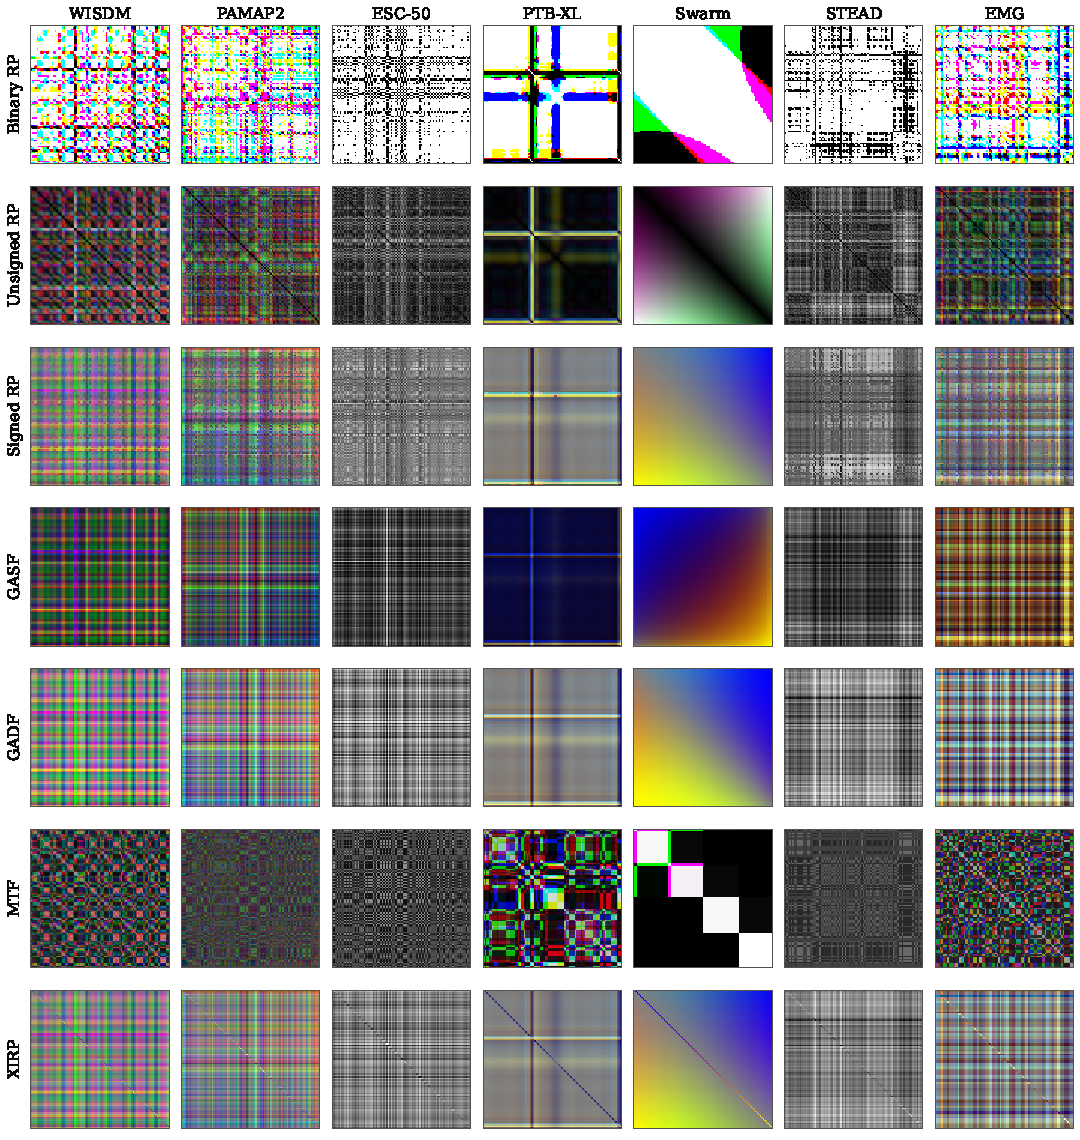
\includegraphics[width=\textwidth]{images/encoding_examples.pdf}
\caption{Representative 8-bit encoding images ($T=128$; one window per dataset). Each channel is stored as its own single-channel image; for display, the first three channels are shown as the red, green and blue planes of one picture, and the single-channel ESC-50 appears in grey. The binary RP uses a recurrence rate of $0.75$. The red (first) channel is decoded in Figure~\ref{fig:examples}.}\label{fig:encodings}
\end{figure}

\begin{table}[!htbp]
\centering
\caption{Information retained by each encoding and reconstruction approaches evaluated. Exactness refers to unquantised matrices under the stated conditions; decoders use the image alone. The geometric, boundary-anchor and spectral decoders and the sign selection of Hirata and Sipers are ours (Section~\ref{sec:methods}); Sipers reads the circular RP.}\label{tab:contract}
\footnotesize
\setlength{\tabcolsep}{4pt}
\begin{tabular}{@{}llll@{}}
\toprule
Encoding & Image retains & Exact recovery & Decoders \\
\midrule
Binary RP & Neighbourhoods & No & Hirata~\cite{hirata2008reproduction} \\
Unsigned RP & State geometry & Up to sign, (a)--(b) & Hirata; Sipers~\cite{sipers2017robust}; geometric \\
Signed RP & Geometry, direction & Prop.~\ref{prop:rp} & Hirata; Sipers; geometric \\
GASF & Angular sums & On $[0,1]$ & Diagonal inverse~\cite{wang2015encoding} \\
GADF & Angular differences & If $\alpha<1/\sqrt2$ & Boundary anchor \\
MTF & State transitions & No & Spectral representative \\
XIRP & Diagonal values & Yes & Inversion by mean~\cite{hellermann2026imagegan} \\
\bottomrule
\end{tabular}
\end{table}

\FloatBarrier
\section{Decoders}\label{sec:methods}

The previous section describes what each encoding retains; here we describe how that information is used to reconstruct a trajectory. All methods operate on the stored image. Published methods are distinguished from our adaptations, and the RP experiments compare both changes of encoded information and changes of decoder.

\subsection{Storage and image-only decoding}\label{sec:storage}

An encoded matrix $M$ is converted to an 8-bit image through the storage rule $\mathcal Q_m(M)=\operatorname{round}\bigl(255\,(M-a)/(b-a)\bigr)$, and the decoder reads $a+(b-a)\,I/255$. GASF and GADF use the known range $[a,b]=[-1,1]$, MTF uses $[0,1]$, and XIRP uses $[1,2]$ on the diagonal and $[-\log2,\log2]$ off it, each with its own map. For signed RP, $[a,b]$ is the min--max of the matrix itself, which contains $0$ because the diagonal is zero and some entry is negative (Eq.~\eqref{eq:signed_rp}). This range is not supplied to the decoder; the quantised diagonal identifies the zero level; subtracting its median recovers a signed matrix up to an unknown positive factor. The subsequent geometric steps and final range normalisation are invariant to this factor. All choices needed to decode the \emph{normalised} trajectory are therefore made from the stored image and globally fixed method settings, not from the original window.

\subsection{Geometric reconstruction of signed RP}\label{sec:rp_decoder}

The proposed decoder recovers state geometry from distances, finds the orientation compatible with consecutive overlapping states, and finally uses directional signs to resolve the remaining reflection. For a length-$T$ signal, the procedure is:
\begin{enumerate}
\item \emph{Distance recovery.} Re-centre the stored 8-bit image $I_{\mathrm{RP}}$ at its diagonal zero level and symmetrise the absolute values:
\[
R^{\mathrm{obs}}=I_{\mathrm{RP}}-\operatorname{median}_i(I_{\mathrm{RP}})_{ii}\,\mathbf1\mathbf1^\top,\qquad
D_{ij}=\frac{|R^{\mathrm{obs}}_{ij}|+|R^{\mathrm{obs}}_{ji}|}{2}.
\]
\item \emph{State geometry.} Apply classical multidimensional scaling~\cite{Torgerson1952}. With $J=I-\mathbf1\mathbf1^\top/(T-1)$ and $D^{\circ2}$ the elementwise square of $D$, form $B=-\tfrac12JD^{\circ2}J$. Its two leading eigenpairs give $Y=V_2\Lambda_2^{1/2}\in\mathbb R^{(T-1)\times2}$, a state configuration determined up to an orthogonal transformation.
\item \emph{Overlap-compatible orientation.} Adjacent states must share one sample: for oriented rows $(a_i,b_i)=(Y_{i1},Y_{i2})\,Q$, ideally $b_i=a_{i+1}$. Parameterise the unknown orthogonal transform by $Q=\operatorname{rot}(\theta)\operatorname{diag}(1,\eta)$, $\eta\in\{-1,+1\}$, with $\operatorname{rot}(\theta)=\bigl(\begin{smallmatrix}\cos\theta&-\sin\theta\\ \sin\theta&\cos\theta\end{smallmatrix}\bigr)$. For each $\eta$, the residual has the form $b_i-a_{i+1}=A_i\cos\theta+B_i\sin\theta$, $i=1,\ldots,T-2$, with
\[
A_i=\eta Y_{i2}-Y_{i+1,1},\qquad
B_i=-\eta Y_{i1}-Y_{i+1,2}.
\]
Removing the mean residual centres both coefficients, $\tilde A_i=A_i-\operatorname{mean}_kA_k$ and $\tilde B_i=B_i-\operatorname{mean}_kB_k$, and the least-squares problem reduces to $\min_{\|u\|=1}u^\top H_\eta u$, where $u=(\cos\theta,\sin\theta)$ and $H_\eta=\tilde C^\top\tilde C$, $\tilde C=[\tilde A\ \tilde B]$. The smallest-eigenvalue eigenvector of each $2\times2$ matrix, taken with both signs, gives four candidates; all four are kept.
\item \emph{Sample assembly.} For each candidate, let $\delta^\star=-\operatorname{mean}_i(b_i-a_{i+1})$ and correct $a_i\mapsto a_i-\delta^\star/2$, $b_i\mapsto b_i+\delta^\star/2$. Set $\hat x_1=a_1$, $\hat x_i=(b_{i-1}+a_i)/2$ for $2\le i\le T-1$, and $\hat x_T=b_{T-1}$, and map its range to $[0,1]$.
\item \emph{Directional disambiguation.} Re-encode each of the four assembled series with Eq.~\eqref{eq:signed_rp} and select the one whose unit-norm signed RP is closest in Frobenius norm to the unit-norm $R^{\mathrm{obs}}$ of step~1. The candidates are compared as assembled series, whose states satisfy the overlap by construction, so on exact input only $\pm x$ can reproduce $R^{\mathrm{obs}}$; a state configuration with its two coordinates swapped, which has the same signed RP as the true states, is never compared directly. This comparison uses the image itself, never the original signal; the selected series is the output $\hat z$.
\end{enumerate}
The orientation problem is linear in $T$, while a dense eigendecomposition dominates the implementation cost, $O(T^3)$.

\subsection{RP baselines and controlled comparisons}\label{sec:hirata}

\paragraph{Geometric decoder without sign}
To isolate the information contributed by directional labels, we also apply the geometric procedure to unsigned distances. We retain the MDS, overlap-fitting and sample-assembly steps, but cannot perform the signed-image comparison. Instead, it returns the candidate with the smallest overlap residual, which selects the parity $\eta$ whose $H_\eta$ has the smaller minimum eigenvalue; the two signs of that eigenvector tie, and the decoder keeps the sign returned by the eigensolver, an arbitrary choice. On non-degenerate exact inputs, both orientations have the same distance image, so an image-only decoder cannot determine which one produced the original.

\paragraph{Hirata et al}
As a binary-RP reference, we implement the graph-distance and MDS construction of Hirata et al.~\cite{hirata2008reproduction,hirata2016chromosome}. Thresholding gives a recurrence graph with edges $B_{ij}=1$. For neighbour sets $G_i=\{k:B_{ik}=1\}$, an edge receives weight $1-|G_i\cap G_j|/|G_i\cup G_j|$; $G_i$ contains $i$, because the binary RP has a unit diagonal. All-pairs shortest paths provide estimated distances, followed by MDS; pairs left unreachable, which can occur at low recurrence rates, are given distance $0$. Converting the resulting coordinates into a length-$T$ series is our post-processing: retain the leading coordinate, append its mean, and rescale the range. We set the recurrence rate to $0.75$ before benchmarking and report a sensitivity analysis over $0.02$--$0.75$ (Section~\ref{sec:results_rp}). When starting from a signed RP, the graph is built by thresholding $|R^{\mathrm{obs}}|$ of step~1 at the same rate; its directional signs are used only in an additional orientation-selection step, which re-encodes $\hat x$ and $-\hat x$, each mapped to the unit range, as signed RPs and keeps the one closer to $R^{\mathrm{obs}}$ with the criterion of step~5 of Section~\ref{sec:rp_decoder}. To check that the one-coordinate post-processing does not drive the comparison, we also passed the same geodesic distances through steps~2--4 of our decoder (up to \binaryWindows{} windows per dataset and length, reflection fixed with the original series in both): the two conversions give an NMAE between \binaryOracleMin{} and \binaryOracleMax{} and differ by at most \binaryGapMax{} in every block, so the loss on the binary RP comes from thresholding, not from the conversion to samples.

\paragraph{Sipers et al}
For continuous unsigned RP, we implement the spectral method of Sipers et al.~\cite{sipers2017robust}. It exploits the factorisation of two-dimensional Fourier coefficients of the squared distance matrix and reconstructs the signal up to a sign. The published construction assumes periodicity, so we provide it with a \emph{circular} RP that includes the wraparound state $(x_T,x_1)$. Image-derived frequency components below $10^{-4}$ of the strongest estimated power are discarded; this threshold was first chosen in an exploratory sweep on evaluated windows and then confirmed on calibration windows outside the evaluated samples, available for six of the seven datasets (Supplementary Sections~\ref{S-sec:s_sipers} and~\ref{S-sec:s_calibration}). Signed RP reconstruction adds our directional orientation-selection step: $\hat x$ and $-\hat x$, mapped to the unit range, are re-encoded as circular signed RPs and the one closer to the observed image in unit-norm Frobenius distance is kept.

\paragraph{Pairing of the comparisons}
Every combination is evaluated on the same windows and channels, so all comparisons are paired by series. Hirata's reconstruction and the geometric decoder, with and without sign, read the same conventional RP image; Sipers' reconstruction reads the circular RP, a different image of the same series. Only Supplementary Table~\ref{S-tab:s_sipers}, where both decoders read the identical circular image, isolates the decoder from the encoding.

\subsection{Restricted-range GADF decoder}\label{sec:gadf_decoder}

GADF provides angular differences but no absolute angle. Our procedure reconstructs a reference angle from the image and then recovers the remaining angles from relative differences. The method assumes the fixed normalisation $[-\alpha,\alpha]$ with $\alpha=0.7<1/\sqrt2$.
\begin{enumerate}
\item \emph{Image-derived boundary anchor.} Compute row means
\[
\mu_i=\frac1T\sum_jG^{\mathrm D}_{ij}=\rho\sin(\phi_i-\psi),
\]
where $\rho\ge0$ and $\psi$ lies within the angular interval spanned by the samples. That interval is narrower than $\pi/2$, so the row means are monotone in $\phi_i$. Thus $e=\arg\max_i|\mu_i|$ is an endpoint sample. Fix $\phi_e=\arccos(-\alpha)$ when $\mu_e>0$ and $\phi_e=\arccos\alpha$ otherwise. Both endpoints are attained in every calibrated window, so either is a valid anchor: when $|\mu_i|$ ties at the two ends, as on a window whose angles are balanced around $\psi$, the choice between them does not matter, and the sign of $\mu_e$, which assigns the angle, cannot be in doubt because $|\mu_e|$ is the largest row mean.
\item \emph{Relative-angle recovery.} For pivot row $p$, recover every angle by
\[
\hat\phi_j^{(p)}=\phi_e-\arcsin G^{\mathrm D}_{ep}-\arcsin G^{\mathrm D}_{pj}.
\]
\item \emph{Quantisation mitigation.} Average the angle estimates obtained from the five rows with the smallest $|\mu_p|$, then return $\hat z_j=\cos\!\bigl(\frac15\sum_p\hat\phi_j^{(p)}\bigr)$, which $\mathcal N_{\mathrm{GADF}}^{-1}$ maps to physical units. The arguments of $\arcsin$ are clipped to $[-1,1]$; the angles are not, so after storage $\hat z_j$ may leave $[-\alpha,\alpha]$ slightly.
\end{enumerate}
The anchor relies on the per-window min--max normalisation, which places a sample at each endpoint; GASF and XIRP read each value from the diagonal and do not need this. A matrix whose angles do not reach $\pm\alpha$, such as one produced by a generative model, would be decoded with a common angular offset, and storage error in the anchor row enters every sample in the same way.
The rows with the smallest $|\mu_p|$ have $\phi_p$ near $\psi$, inside the angular interval. Routing every sample through such a pivot splits each angular difference into two shorter hops, whereas a single hop from the anchor to the opposite endpoint spans nearly $\pi/2$ (about $1.55$ for $\alpha=0.7$), where $|G^{\mathrm D}|\to1$ and the derivative of $\arcsin$ amplifies quantisation error.
Under the normalisation assumptions the decoder is exact before storage and has $O(T^2)$ complexity. The invertibility follows from the restricted normalisation; an elementary inversion of relative angles would still need one absolute angle from outside the image. Our contribution is to take that angle from the image, through the endpoint anchor, and to average over central pivots, a numerical choice against quantisation rather than a condition for identifiability.

\subsection{GASF, MTF and XIRP reference decoders}

\paragraph{GASF} We apply the established diagonal inverse on the $[0,1]$ domain~\cite{wang2015encoding}. Its error after 8-bit storage can therefore be distinguished from the exact-input inverse.

\paragraph{MTF} Since the image does not identify within-state amplitudes, our decoder constructs a representative sequence rather than an exact inverse. In a noiseless MTF all samples of one state have identical rows, so the $T$ image rows, normalised to unit length, are grouped into $Q=4$ clusters by $k$-means with cosine similarity, the same number of quantile states as the encoder and a value fixed in advance (Supplementary Section~\ref{S-sec:s_params}). We estimate the transition matrix $\hat W$ from the means of the corresponding image blocks, normalised by rows, and order the clusters using the Fiedler vector of the unnormalised Laplacian $\operatorname{diag}(S\mathbf1)-S$ of $S=(\hat W+\hat W^\top)/2$~\cite{Atkins1998}. State $k$ is assigned the bin midpoint $(k-\tfrac12)/Q$, and $\mathcal N^{-1}_{\mathrm{MTF}}$ maps $[0,1]$ to $[x_{\min},x_{\max}]$, so the output spans the central $75\%$ of the range; uniform midpoints also ignore that the states are quantiles, an approximation whenever the amplitudes are not uniformly distributed. The Fiedler vector is defined only up to sign, so the order may be reversed, which reflects the series; the decoder does not attempt to resolve this. Neither absolute state order nor within-state amplitudes are guaranteed by the image, so the resulting error combines irreversible encoding loss with approximation choices of the decoder.

\paragraph{XIRP} We use the inversion-by-mean procedure of Hellermann and Lessmann~\cite{hellermann2026imagegan}, which averages the proposals of every column, $\hat z_i=\frac1T\bigl(\hat R_{ii}+\sum_{j\ne i}\hat R_{jj}\exp(\hat R_{ij})\bigr)$ on the stored matrix $\hat R$. Since the original normalised values appear on the matrix diagonal, this method serves as an invertible reference whose remaining error after quantisation can be measured directly.

% ============================================================================================
\section{Experimental protocol}\label{sec:protocol}

\subsection{Datasets and windows}
Table~\ref{tab:datasets} lists the seven public datasets: human activity (WISDM~\cite{misc_wisdm_smartphone_and_smartwatch_activity_and_biometrics_dataset__507}, PAMAP2~\cite{reiss2012pamap2}), environmental audio (ESC-50~\cite{piczak2015esc}), electrocardiography (PTB-XL~\cite{wagner2020ptbxl}), geomagnetism (Swarm~\cite{friis2006swarm}), seismology (STEAD~\cite{mousavi2019stead}) and surface electromyography (EMG~\cite{krilova2018emg}). Every channel is encoded, stored and decoded as its own single-channel image with its own calibration. Recordings are cut into non-overlapping windows of $T\in\{64,128,256\}$ samples that never cross a label change or a time gap. Blocks with fewer than 200 windows (EMG at $T=256$) are not reported. Preprocessing and sample sizes are detailed per dataset in Supplementary Section~\ref{S-sec:s_datasets}.

\begin{table}[!htbp]
\centering
\caption{Datasets. Windows of 128 samples available after segmentation, after the resampling and record selection of Supplementary Section~\ref{S-sec:s_datasets} (ESC-50 resampled from 44.1\,kHz, 3\,000 PTB-XL records, January 2023 for Swarm, 2\,000 STEAD traces). The group (for ESC-50, the Freesound source recording) is the unit that never appears on both sides of a split; in parentheses, the number of groups in the classification sample at $T=128$.}\label{tab:datasets}
\footnotesize
\setlength{\tabcolsep}{4pt}
\begin{tabular}{@{}lrrlrl@{}}
\toprule
Dataset & $f_s$ (Hz) & Channels & Task & Windows & Group \\
\midrule
WISDM & 20 & 3 & 5 activities & 8\,172 & subject (51) \\
PAMAP2 & 100 & 9 & 12 activities & 15\,085 & subject (9) \\
ESC-50 & 8\,000 & 1 & 50 sound classes & 624\,000 & recording (1\,465) \\
PTB-XL & 100 & 12 & 5 multilabel classes & 21\,000 & patient (2\,649) \\
Swarm MAG & 1 & 3 & none & 62\,757 & day \\
STEAD & 100 & 3 & quake vs noise & 92\,000 & event/station (1\,450) \\
EMG gestures & 100 & 8 & 6 gestures & 880 & subject (36) \\
\bottomrule
\end{tabular}
\end{table}

\subsection{Fidelity, robustness and cost}
Fidelity uses 500 windows per dataset and length drawn with a fixed seed, and 3\,000 for the single-channel ESC-50, so that every block holds between about 1\,500 and 6\,000 channel series. Writing $r=\max_ix_i-\min_ix_i$, it is measured per channel series by
\[
\mathrm{NMAE}=\frac{1}{rT}\sum_i|x_i-\hat x_i|,
\]
the Pearson correlation, the $L_1$ distance between unit-mass Welch spectra~\cite{Welch1967} and the relative energy error $|\sum_fP_{\hat x}(f)-\sum_fP_x(f)|/\sum_fP_x(f)$; constant series are excluded. Spectra use Hann segments of $\max(16,T/2)$ samples with $50\%$ overlap, and the mean of each segment is removed, so the energy error concerns the fluctuations, not the mean level. Each decoder is run on the floating-point matrix and on the 8-bit image. Robustness adds zero-mean Gaussian noise of $\sigma\in\{2,4,8,16\}$ intensity levels to every pixel of the stored image, which is then clipped and rounded, with two replicates per level on 200 windows per dataset and length. Cost is the single-thread time to encode, store and decode and the peak traced memory, for $T$ from 64 to 1\,024. The sampling-rate study reads 3\,000 PTB-XL records at 500\,Hz and resamples them with an anti-aliased polyphase filter to 250, 100 and 50\,Hz, with windows of 128 samples and, as a control, of a fixed duration of 1.28\,s.

\subsection{Classification utility}
Classifiers are trained on original windows and evaluated on the original and on every reconstruction of the same held-out windows. Up to 6\,000 windows per dataset and length are split into three grouped folds that keep every subject, patient, event, station or source recording on one side, stratified by class for single-label data; per-channel standardisation uses training statistics only, and reconstructions are produced independently per window, so no information crosses the split. KNN, an RBF SVM, a random forest, an LSTM, a GRU and a one-dimensional CNN are used with standard settings (Supplementary Section~\ref{S-sec:s_classifiers}). Accuracy, or macro-F1 for the multilabel PTB-XL, is averaged over the three folds. Swarm has no labels. At 8\,kHz, ESC-50 windows of 128 samples span 16\,ms of sound, which leaves every classifier near chance, so audio is evaluated on the official ESC-10 subset at 2, 4 and 8\,kHz with windows of 512 and 1\,024 samples, silent windows removed and accuracy scored per clip, by averaging the class probabilities of the clip's windows.

\subsection{Statistical protocol}
All comparisons are paired over the same series; differences between decoders are summarised by medians of per-series differences, averaged across datasets with equal weight. A reconstruction is declared \emph{equivalent} to the original for a classifier when the $95\%$ bootstrap interval of the accuracy difference, resampling whole groups~\cite{DavisonHinkley1997,Hall1987}, lies within $\pm0.01$, which corresponds to two one-sided tests at the $2.5\%$ level~\cite{Schuirmann1987,Lakens2017}; a non-significant difference is not taken as evidence of equivalence. The difference is computed per group on the out-of-fold predictions and averaged over groups without weights, so it can differ from the window-weighted fold means of Table~\ref{tab:utility}; the interval is the percentile interval of 2\,000 resamples of the groups. The interval treats groups as independent, although their predictions come from three models with overlapping training data, and with few groups, such as the nine PAMAP2 subjects, a percentile cluster bootstrap can understate the uncertainty, so equivalence on such datasets is weaker evidence. Equivalence is assessed on single-label data; for PTB-XL only the drop in macro-F1 is reported.

% ============================================================================================
\FloatBarrier
\section{Results}\label{sec:results}

\subsection{Fidelity and storage (RQ1)}\label{sec:results_fidelity}
Table~\ref{tab:fidelity} gives the 8-bit error of every combination at $T=128$; the other lengths behave alike (Supplementary Tables~\ref{S-tab:s_l64} and~\ref{S-tab:s_l256}). Over the \benchBlocks{} reported dataset--length blocks, \benchSeries{} channel series were reconstructed by every combination without decoder failure.

On the floating-point matrix, the geometric decoder on the signed RP, GASF, GADF and XIRP recover the series to machine precision: over every series of every block, the largest error is \floatWorstRP{} for the signed RP and \floatWorstGASF, \floatWorstGADF{} and \floatWorstXIRP{} for GASF, GADF and XIRP. For these four, the 8-bit error is therefore storage error. Over the \benchBlocks{} blocks of all three lengths, its mean stays between \rpEightMin{} and \rpEightMax{} for the signed RP on six datasets and rises to \rpEightSwarmMin--\rpEightSwarmMax{} on Swarm; GASF and GADF are of the same order, and XIRP is about an order of magnitude lower. Sipers' reconstruction on the circular signed RP comes close, between \sipEightMin{} and \sipEightMax{} over the same blocks; with its frequency threshold it is not exact in floating point (median error up to \floatMaxSIPERS{} per block; Supplementary Section~\ref{S-sec:s_sipers}). The per-series error is skewed, and on the unsigned RP bimodal, depending on whether the reflection is returned; Supplementary Table~\ref{S-tab:s_spread} gives its median and interquartile range at $T=128$.

The remaining combinations reach a mean NMAE between about $0.03$ and $0.34$ over all blocks, for two different reasons (Figure~\ref{fig:examples}; spectral and correlational metrics in Supplementary Table~\ref{S-tab:s_spectral}). On the unsigned RP, the geometric and Sipers' decoders keep the spectrum as well as on the signed RP, because a reflection leaves the spectrum unchanged; their pointwise error and their correlation of about zero come from returning the reflection in about half of the series. Hirata's reconstruction and the MTF representative also distort the spectrum and the energy: they lose the waveform, not only its sign.
\begin{table}[!htbp]
\centering
\caption{Mean 8-bit NMAE of every encoding--decoder combination at $T=128$ (500 windows per dataset, 3\,000 for ESC-50; every channel). Uns./Sig.: unsigned and signed RP. Sipers' decoder reads the circular RP, a different image from the conventional RP read by the other RP decoders (Section~\ref{sec:hirata}); Supplementary Table~\ref{S-tab:s_sipers} compares the decoders on the same image. Per-series medians and interquartile ranges: Supplementary Table~\ref{S-tab:s_spread}.}\label{tab:fidelity}
\scriptsize
\setlength{\tabcolsep}{2.5pt}
\begin{tabular}{@{}lrrrrrrrr@{}}
\toprule
Dataset & Hirata\,/\,uns. & Hirata\,/\,sig. & Ours\,/\,uns. & Ours\,/\,sig. & GASF & GADF & MTF & XIRP \\
\midrule
WISDM & 0.2411 & 0.1044 & 0.1946 & 0.0010 & 0.0015 & 0.0013 & 0.2838 & 0.0002 \\
PAMAP2 & 0.2345 & 0.1059 & 0.1899 & 0.0015 & 0.0016 & 0.0013 & 0.2771 & 0.0002 \\
ESC-50 & 0.2177 & 0.0830 & 0.1747 & 0.0018 & 0.0016 & 0.0010 & 0.2725 & 0.0002 \\
PTB-XL & 0.3313 & 0.1982 & 0.2874 & 0.0016 & 0.0029 & 0.0023 & 0.3404 & 0.0002 \\
Swarm & 0.2778 & 0.0283 & 0.2547 & 0.0124 & 0.0026 & 0.0015 & 0.2979 & 0.0002 \\
STEAD & 0.2044 & 0.0868 & 0.1771 & 0.0013 & 0.0015 & 0.0011 & 0.2668 & 0.0002 \\
EMG & 0.1979 & 0.1205 & 0.1680 & 0.0009 & 0.0013 & 0.0022 & 0.2834 & 0.0006 \\
\bottomrule
\end{tabular}

\end{table}

\subsection{Recurrence plots: encoding versus decoder (RQ2)}\label{sec:results_rp}
Table~\ref{tab:fidelity} separates five effects. The spectrum is unchanged by a reflection of the series, so it shows what each decoder keeps of the waveform independently of its orientation. \emph{Sign.} On the unsigned RP, the geometric decoder keeps the spectrum as well as on the signed RP (PSD-shape distance \psdGeoUnsMin--\psdGeoUnsMax{}, against \psdGeoSigMin--\psdGeoSigMax{}), while its correlation with the original stays within $\pm$\pearsonUnsAbsMax{}: it recovers the shape and loses only the orientation, which the sign restores from the image alone (Figure~\ref{fig:examples}). \emph{Thresholding.} Hirata's reconstruction from the binarised RP distorts the spectrum itself (\psdHirMin--\psdHirMax{}): once the image is binary, the waveform is lost, not only its sign. \emph{Information and algorithm.} On the same signed RP, the geometric decoder is one to two orders of magnitude more accurate than Hirata's on six datasets; on Swarm the gap narrows to a factor of about two. This comparison changes both the information used, continuous distances against a thresholded graph, and the algorithm, two-dimensional MDS with overlap assembly against graph geodesics with our one-coordinate post-processing, so the gap cannot be attributed to the distances alone. The conversion to samples is not what separates them: on the same geodesic distances, our assembly and Hirata's one-coordinate post-processing differ by at most \binaryGapMax{} (Section~\ref{sec:hirata}). \emph{Decoder on continuous distances.} Sipers' reconstruction also uses the continuous distances; with the sign it is a median of \macroDiffRPSIPERSSIGNED{} per series above the geometric decoder, which on the same circular image is \pilotRatioMin{} to \pilotRatioMax{} times more accurate on every dataset (Supplementary Table~\ref{S-tab:s_sipers}). It is ahead in the benchmark only on Swarm, and the gain comes from the encoding. On the 100 Swarm windows of that paired comparison (means, so slightly different from Table~\ref{tab:fidelity}), adding the wrap state raises the median $\sigma_2/\sigma_1$ from \swRatioNonCirc{} to \swRatioCirc{} and lowers the geometric decoder's error from \swGeoNonCirc{} to \swGeoCirc{}, below Sipers' \swSipCirc{} on the same image, while on other datasets it changes by at most \encGapMax{}. \emph{Threshold choice.} These comparisons do not depend on the recurrence rate fixed for Hirata: choosing the best rate per dataset with knowledge of the result lowers its error by at most \hirataGainUns{} on the unsigned and \hirataGainSig{} on the signed RP, leaving it between \hirataBestMin{} and \hirataBestMax{} (Supplementary Table~\ref{S-tab:s_hirata}).

\begin{figure}[!htbp]
\centering
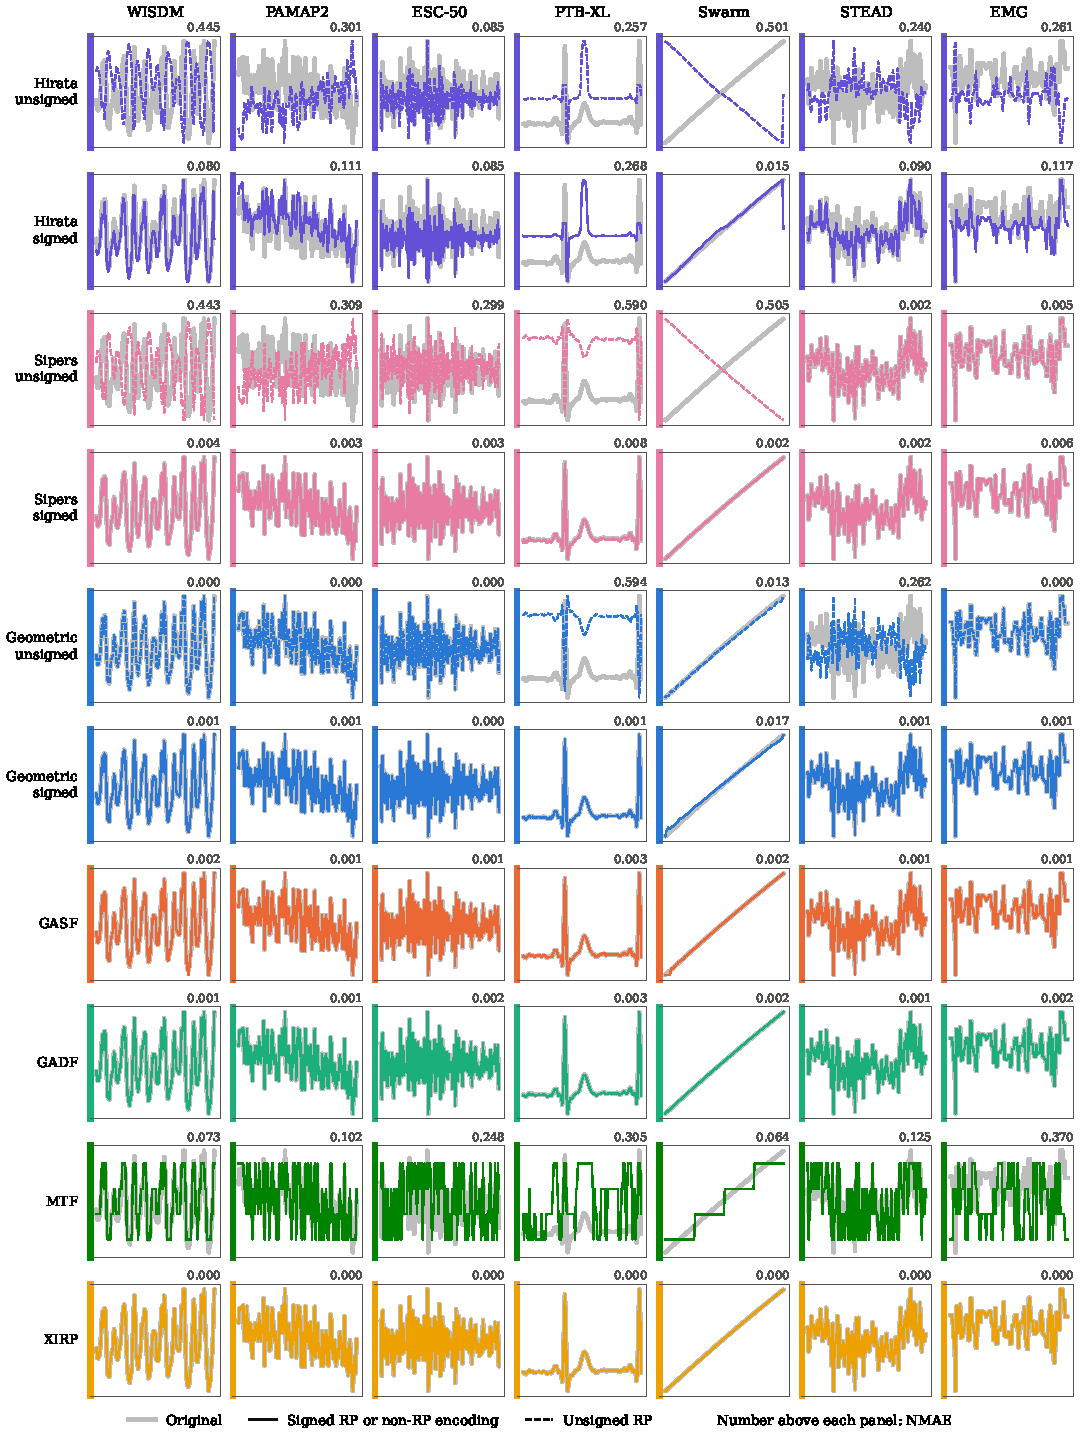
\includegraphics[width=\textwidth,height=0.78\textheight,keepaspectratio]{images/reconstruction_examples.pdf}
\caption{The first channel of the windows of Figure~\ref{fig:encodings}, decoded from its 8-bit image. Each row is one encoding--decoder combination, in the order of Table~\ref{tab:fidelity}, and each column one dataset; the original is the grey band, the reconstruction is drawn on top of it, and the NMAE of the panel is given above it. On Swarm, whose states are nearly collinear, the signed RP deviates visibly at the start of the window.}\label{fig:examples}
\end{figure}

\subsection{Signal characteristics and stability (RQ3)}\label{sec:results_conditions}
As the eigengap argument of Section~\ref{sec:rp_encodings} anticipates, storage error grows when the states are nearly collinear. None of the \condGoodSeries{} series with $\sigma_2/\sigma_1\ge0.1$ exceeds an 8-bit NMAE of $0.01$, whereas \condWorstRate\% of the series with $\sigma_2/\sigma_1<0.01$ do. The ratio is an empirical indicator, not a complete explanation: it separates the regimes at the two ends but does not determine which series in between fail. Nor does the share of sign-informative pairs: slow series are informative in nearly every pair, yet their states are the most collinear. Swarm, sampled at 1\,Hz, is the limiting case and the only dataset where the signed RP is not in the low-error group.

The sampling rate changes how far apart consecutive samples are, and with it the conditioning (Figure~\ref{fig:robustness_sampling}b--c). On PTB-XL with windows of 128 samples, from 50 to 500\,Hz the median $\sigma_2/\sigma_1$ falls from \srColFifty{} to \srColFivehundred{}, the share of series below $0.1$ grows from \srShareFifty\% to \srShareFivehundred\%, and the 8-bit NMAE of the signed RP rises from \srRPFifty{} to \srRPFivehundred{}, while GASF and GADF stay between \srGafMin{} and \srGafMax{} and XIRP is unaffected. A fixed number of samples spans a shorter time at a higher rate, but the trend persists at a fixed duration of 1.28\,s, from \srDurRPFifty{} to \srDurRPFivehundred{} (Supplementary Table~\ref{S-tab:s_sampling}). Sipers' reconstruction rises with the rate as well (Figure~\ref{fig:robustness_sampling}b), so the effect belongs to the RP, not to one decoder. On the 3\,000 records of this study, the resampled and the distributed 100\,Hz files give the same mean error (\srResampledRP{} and \srNativeRP{}; Table~\ref{tab:fidelity} uses a different sample of windows). Resampling also changes the spectral content of each window, and the study covers one dataset, so the trend is attributable to the rate as realised by anti-aliased resampling of PTB-XL, not to the rate in isolation.

\begin{figure}[!htbp]
\centering
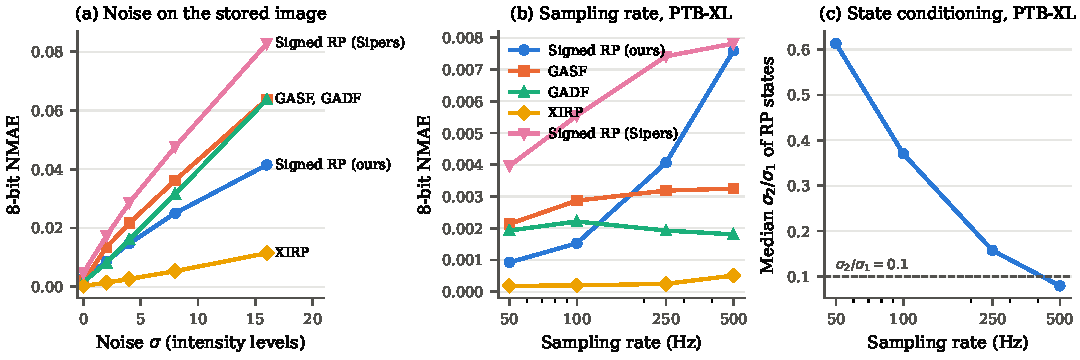
\includegraphics[width=\textwidth]{images/robustness_sampling.pdf}
\caption{(a) Mean 8-bit NMAE against Gaussian noise added to the stored image ($T=128$, mean over the seven datasets, two replicates per level). (b) 8-bit NMAE and (c) median conditioning $\sigma_2/\sigma_1$ of the RP states against the sampling rate (PTB-XL, $T=128$, anti-aliased resampling from 500\,Hz). Hirata's reconstruction, the geometric and Sipers' decoders on the unsigned RP and MTF stay between 0.08 and 0.34 throughout and are omitted.}\label{fig:robustness_sampling}
\end{figure}

\subsection{Classification utility (RQ4)}
Six classifiers, five labelled datasets and three lengths give \clsCombos{} combinations on \clsWindows{} windows (Table~\ref{tab:utility}). On the original windows, accuracy ranges from \origAccMin{} to \origAccMax{} and PTB-XL macro-F1 from \origFoneMin{} to \origFoneMax{}; the lowest values (KNN on EMG) are near chance, where drops are less informative. The four combinations that are exact in floating point never lose more than \clsMaxDropExact{} and are equivalent within $\pm0.01$ in nearly every single-label combination; where equivalence is not established, the observed difference is still below $0.01$ and the interval is too wide rather than the drop large. Sipers' reconstruction on the circular signed RP joins this group, with a largest drop of \sipersSigMaxDrop{}, but is equivalent in fewer combinations (\sipersSigEq{} of \clsCombosEq{}, against \clsEqRP{} for the geometric decoder), consistent with its larger 8-bit error. Without the sign, Sipers' reconstruction, Hirata's on either encoding, the geometric decoder on the unsigned RP and MTF lose between $0.08$ and $0.12$ on average and up to $0.40$: whichever decoder is used, the unsigned RP loses the orientation and with it the accuracy. The same separation holds per clip on ESC-10 (\escWindows{} windows, \escCombos{} combinations), where the exactly decodable combinations lose at most \escMaxDropExact{}. Results per dataset and per ESC-10 block are in Supplementary Section~\ref{S-sec:s_classification}.

\begin{table}[!htbp]
\centering
\caption{Drop from the original accuracy (macro-F1 on PTB-XL) for classifiers trained on original windows and tested on reconstructions. $|\Delta|\le0.01$: share of combinations whose observed drop is within $0.01$. Equivalent: $95\%$ group-bootstrap interval within $\pm0.01$, over the single-label combinations.}\label{tab:utility}
\footnotesize
\setlength{\tabcolsep}{3pt}
\begin{tabular}{@{}lrrrrrr@{}}
\toprule
& \multicolumn{4}{c}{Six datasets, $T\in\{64,128,256\}$} & \multicolumn{2}{c}{ESC-10, per clip} \\
\cmidrule(lr){2-5}\cmidrule(l){6-7}
Decoder & Mean drop & Max drop & $|\Delta|\le0.01$ & Equivalent & Mean drop & Equivalent \\
\midrule
Hirata\,/\,uns. & 0.120 & 0.376 & 19\% & 11/66 & 0.071 & 0/36 \\
Hirata\,/\,sig. & 0.080 & 0.283 & 26\% & 12/66 & 0.060 & 0/36 \\
Ours\,/\,uns. & 0.099 & 0.359 & 21\% & 13/66 & 0.024 & 0/36 \\
Ours\,/\,sig. & 0.000 & 0.007 & 100\% & 63/66 & 0.001 & 33/36 \\
GASF & -0.000 & 0.005 & 100\% & 63/66 & 0.001 & 34/36 \\
GADF & -0.000 & 0.002 & 100\% & 63/66 & 0.000 & 32/36 \\
MTF & 0.099 & 0.400 & 19\% & 7/66 & 0.106 & 0/36 \\
XIRP & 0.000 & 0.002 & 100\% & 65/66 & -0.000 & 36/36 \\
\bottomrule
\end{tabular}

\end{table}

\subsection{Robustness (RQ3) and cost (RQ4)}
With noise of $\sigma=16$ intensity levels on the stored image, the mean NMAE at $T=128$ rises to \robHighXIRP{} for XIRP, \robHighRP{} for the signed RP, \robHighGASF{} for GASF, \robHighGADF{} for GADF and \robHighSIPERS{} for Sipers' reconstruction on the circular signed RP (Figure~\ref{fig:robustness_sampling}a). The geometric decoder on the signed RP degrades less than both angular fields on \robDatasetsRPBetter{} of the \robDatasets{} datasets, with all three at a similar level on Swarm, and less than Sipers' on \robDatasetsRPBetterSipers{} of the \robDatasets{}. The lossy combinations move by at most \robLossyShift{}, because their error is already dominated by what is discarded before storage. Supplementary Table~\ref{S-tab:s_robustness} gives every dataset.

Hirata's reconstruction has the steepest cost, with an exponent of about $2.6$ due to all-pairs shortest paths (Supplementary Table~\ref{S-tab:s_cost}); this applies to the geodesic formulation evaluated here, not to the later linear-time refinement of Hirata et al.~\cite{hirata2021fast}, which we did not evaluate. The geometric decoder on the signed RP is \speedupMid{} times faster at $T=256$ and \speedupLong{} times faster at $T=1024$, and costs about as much as Sipers' reconstruction at $T=256$ and half as much at $T=1024$. GASF, GADF, XIRP and MTF are one to two orders of magnitude cheaper. Memory grows quadratically for all of them.
% ============================================================================================
\FloatBarrier
\section{Discussion}\label{sec:discussion}

\paragraph{Invertibility is not stability}
Four combinations are exact on unquantised matrices and keep classifier accuracy after 8-bit storage, but exactness before quantisation does not determine how errors propagate afterwards. The signed RP is the clearest case: its storage error follows the conditioning of the states, for Sipers' decoder as for ours, while GASF and GADF stay level. XIRP, whose column proposals are redundant, was the least sensitive to quantisation and to pixel noise; its lower error reflects that it stores the series by design and says nothing about whether its images are better inputs for classification or generation. These observations hold for the storage and perturbations studied here, 8-bit images and independent Gaussian pixel noise; other formats or structured perturbations may behave differently.

\paragraph{What an encoding retains and how well it is decoded are different questions}
The unsigned RP keeps the geometry of the states but not their orientation: both the geometric decoder and Sipers' recover the spectrum and lose the sign, so this loss belongs to the encoding, not to a decoder. The binary RP and MTF are many-to-one, so no decoder can be exact for every series; the evaluated decoders lose most of the waveform, and better approximations, for instance with learned priors, are not ruled out but cannot guarantee the encoded series either. Once the information is present, both the decoder and the encoding matter: on the same image the geometric decoder is more accurate than Sipers', yet circularisation alone was enough to reverse their order on Swarm (Section~\ref{sec:results_rp}). Comparisons between RP decoders should therefore fix the encoding before attributing a difference to the algorithm.

\paragraph{From encoder outputs to generated images}
Every image studied here is the output of a known encoder applied to a real series. Decoding such images does not show that a generator can produce images with the same structure, nor that the series decoded from generated images are good synthetic data. A generated signed RP need not be a signed Euclidean distance matrix with a zero diagonal and consistent signs, a generated GADF need not stay on the restricted branch, and the per-window calibration $(x_{\min},x_{\max})$ would have to be generated or fixed. Hellermann and Lessmann address the first problem by designing XIRP to be invertible~\cite{hellermann2026imagegan}; our results show which other encodings can be decoded once their structure is respected, and under which conditions.

\paragraph{Limitations}
Images are deterministic outputs of known encoders; pixel noise measures local stability only. Physical units need the window's own channel extremes; only 8-bit storage and independent channels are studied. PTB-XL and ESC-50 are split by patient and recording, not by official folds. Both RP baselines are our implementations with thresholds their authors do not fix for our data, and the coarse-to-fine refinement of Hirata et al.~\cite{hirata2021fast} is not evaluated. The sampling-rate study covers one dataset.

\section{Conclusions}\label{sec:conclusions}
Across seven datasets from six domains, the signed recurrence plot with a geometric decoder, GASF on $[0,1]$, GADF on a restricted angular range and XIRP are exactly decodable before quantisation under stated conditions, and after 8-bit storage they keep what classifiers trained on original signals need. The unsigned recurrence plot is recovered only up to a reflection; the binary recurrence plot and the Markov transition field are many-to-one. For recurrence plots, stability after storage depends on the conditioning of the states, which worsened as the sampling rate of PTB-XL grew. A natural line of research is image generation constrained to valid encodings. For the signed RP, a valid image is a signed Euclidean distance matrix with consistent signs whose adjacent states overlap; for GADF, a matrix on the restricted branch. How to enforce these constraints during generation, or to project a generated image onto them, remains open. Series decoded from such images could then be assessed with the fidelity and utility measures used here.

% ============================================================================================
\section*{CRediT authorship contribution statement}
\noindent\textbf{Adriano García-Giralda Milena:} Conceptualization, Methodology, Software, Formal analysis, Investigation, Data curation, Validation, Visualization, Writing -- original draft, Writing -- review \& editing.
\textbf{Francisco García Moreno:} Conceptualization, Methodology, Supervision, Writing -- review \& editing.
\textbf{José Antonio Jiménez Madrid:} Methodology, Formal analysis, Writing -- review \& editing.
\textbf{María Bermúdez Edo:} Supervision, Writing -- review \& editing.

\section*{Funding}
This research did not receive any specific grant from funding agencies in the public, commercial, or not-for-profit sectors.

\section*{Data availability}
All datasets are public and cited. Code, manifests, configurations and derived results are available at\\
\url{https://github.com/adrianoggm/time-series-image-reconstruction}.

\section*{Declaration of generative AI and AI-assisted technologies in the manuscript preparation process}
During the preparation of this work, the authors used Claude Code to support software implementation and debugging, LaTeX formatting, manuscript organisation and language refinement. The authors reviewed and validated all resulting code, procedures and text, and take full responsibility for the methodology, results, interpretations and content of the manuscript.

{\small
\begin{thebibliography}{99}
\setlength{\itemsep}{0pt}
\setlength{\parskip}{0pt}
\raggedright

\bibitem{wang2015encoding}
Zhiguang Wang and Tim Oates. ``Imaging time-series to improve classification and imputation''. In \textit{Proceedings of the 24th International Joint Conference on Artificial Intelligence (IJCAI)}, pp. 3939--3945, 2015.

\bibitem{wang2015encoding2}
Zhiguang Wang and Tim Oates. ``Encoding time series as images for visual inspection and classification using tiled convolutional neural networks''. In \textit{Trajectory-Based Behavior Analytics: Papers from the 2015 AAAI Workshop}, AAAI Technical Report WS-15-14, AAAI Press, 2015.

\bibitem{huang2023tsdigan}
Tongge Huang, Pranamesh Chakraborty, and Anuj Sharma. ``Deep convolutional generative adversarial networks for traffic data imputation encoding time series as images''. \textit{International Journal of Transportation Science and Technology}, vol. 12, no. 1, pp. 1--18, 2023. doi:\url{10.1016/j.ijtst.2021.10.007}.

\bibitem{hellermann2026imagegan}
Justin Hellermann and Stefan Lessmann. ``Leveraging image-based generative adversarial networks for time series generation''. \textit{International Journal of Forecasting}, vol. 42, no. 2, pp. 616--639, 2026. doi:\url{10.1016/j.ijforecast.2025.09.004}.

\bibitem{eckmann1987recurrence}
Jean-Pierre Eckmann, S. Oliffson Kamphorst, and David Ruelle. ``Recurrence plots of dynamical systems''. \textit{Europhysics Letters}, vol. 4, no. 9, pp. 973--977, 1987. doi:\url{10.1209/0295-5075/4/9/004}.

\bibitem{marwan2007recurrence}
Norbert Marwan, M. Carmen Romano, Marco Thiel, and Jürgen Kurths. ``Recurrence plots for the analysis of complex systems''. \textit{Physics Reports}, vol. 438, no. 5--6, pp. 237--329, 2007. doi:\url{10.1016/j.physrep.2006.11.001}.

\bibitem{ahmad2021inertial}
Zeeshan Ahmad and Naimul Khan. ``Inertial sensor data to image encoding for human action recognition''. \textit{IEEE Sensors Journal}, vol. 21, no. 9, pp. 10978--10988, 2021. doi:\url{10.1109/JSEN.2021.3062261}.

\bibitem{ma2024anomaly}
Jidong Ma and Hairu Wang. ``Anomaly detection in sensor data via encoding time series into images''. \textit{Journal of King Saud University -- Computer and Information Sciences}, vol. 36, no. 10, article 102232, 2024. doi:\url{10.1016/j.jksuci.2024.102232}.

\bibitem{huamin2020reconstruction}
Huamin Tao, Qiuqun Deng, and Shanzhu Xiao. ``Reconstruction of time series with missing value using 2D representation-based denoising autoencoder''. \textit{Journal of Systems Engineering and Electronics}, vol. 31, no. 6, pp. 1087--1096, 2020. doi:\url{10.23919/JSEE.2020.000081}.

\bibitem{takens1981detecting}
Floris Takens. ``Detecting strange attractors in turbulence''. In \textit{Dynamical Systems and Turbulence, Warwick 1980}, Lecture Notes in Mathematics, vol. 898, pp. 366--381, Springer, 1981. doi:\url{10.1007/BFb0091924}.

\bibitem{lu2019robust}
Jianjie Lu and Kai-Yu Tong. ``Robust single accelerometer-based activity recognition using modified recurrence plot''. \textit{IEEE Sensors Journal}, vol. 19, no. 15, pp. 6317--6324, 2019. doi:\url{10.1109/JSEN.2019.2911204}.

\bibitem{hirata2008reproduction}
Yoshito Hirata, Shunsuke Horai, and Kazuyuki Aihara. ``Reproduction of distance matrices and original time series from recurrence plots and their applications''. \textit{The European Physical Journal Special Topics}, vol. 164, no. 1, pp. 13--22, 2008. doi:\url{10.1140/epjst/e2008-00830-8}.

\bibitem{thiel2004information}
Marco Thiel, M. Carmen Romano, and Jürgen Kurths. ``How much information is contained in a recurrence plot?''. \textit{Physics Letters A}, vol. 330, no. 5, pp. 343--349, 2004. doi:\url{10.1016/j.physleta.2004.07.050}.

\bibitem{hirata2021fast}
Yoshito Hirata, Yuki Kitanishi, Hiroki Sugishita, and Yukiko Gotoh. ``Fast reconstruction of an original continuous series from a recurrence plot''. \textit{Chaos}, vol. 31, no. 12, article 121101, 2021. doi:\url{10.1063/5.0073899}.

\bibitem{naiman2024imagentime}
Ilan Naiman, Nimrod Berman, Itai Pemper, Idan Arbiv, Gal Fadlon, and Omri Azencot. ``Utilizing image transforms and diffusion models for generative modeling of short and long time series''. In \textit{Advances in Neural Information Processing Systems 37 (NeurIPS 2024)}, 2024. doi:\url{10.52202/079017-3868}.

\bibitem{sipers2011unique}
Aloys Sipers, Paul J. A. Borm, and Ralf L. M. Peeters. ``On the unique reconstruction of a signal from its unthresholded recurrence plot''. \textit{Physics Letters A}, vol. 375, no. 24, pp. 2309--2321, 2011. doi:\url{10.1016/j.physleta.2011.04.040}.

\bibitem{sipers2017robust}
Aloys Sipers, Paul J. A. Borm, and Ralf L. M. Peeters. ``Robust reconstruction of a signal from its unthresholded recurrence plot subject to disturbances''. \textit{Physics Letters A}, vol. 381, no. 6, pp. 604--615, 2017. doi:\url{10.1016/j.physleta.2016.12.028}.

\bibitem{Torgerson1952}
Warren S. Torgerson. ``Multidimensional scaling: I. Theory and method''. \textit{Psychometrika}, vol. 17, no. 4, pp. 401--419, 1952. doi:\url{10.1007/BF02288916}.

\bibitem{Atkins1998}
Jonathan E. Atkins, Erik G. Boman, and Bruce Hendrickson. ``A spectral algorithm for seriation and the consecutive ones problem''. \textit{SIAM Journal on Computing}, vol. 28, no. 1, pp. 297--310, 1998. doi:\url{10.1137/S0097539795285771}.

\bibitem{misc_wisdm_smartphone_and_smartwatch_activity_and_biometrics_dataset__507}
Gary M. Weiss. ``WISDM Smartphone and Smartwatch Activity and Biometrics Dataset''. \textit{UCI Machine Learning Repository}, 2019. doi:\url{10.24432/C5HK59}.

\bibitem{Welch1967}
Peter D. Welch. ``The use of fast Fourier transform for the estimation of power spectra: A method based on time averaging over short, modified periodograms''. \textit{IEEE Transactions on Audio and Electroacoustics}, vol. 15, no. 2, pp. 70--73, 1967. doi:\url{10.1109/TAU.1967.1161901}.

\bibitem{DavisonHinkley1997}
Anthony C. Davison and David V. Hinkley. \textit{Bootstrap Methods and Their Application}. Cambridge University Press, 1997.

\bibitem{Hall1987}
Peter Hall. ``On the bootstrap and likelihood-based confidence regions''. \textit{Biometrika}, vol. 74, no. 3, pp. 481--493, 1987. doi:\url{10.1093/biomet/74.3.481}.

\bibitem{Lakens2017}
Daniël Lakens. ``Equivalence tests: A practical primer for t tests, correlations, and meta-analyses''. \textit{Social Psychological and Personality Science}, vol. 8, no. 4, pp. 355--362, 2017. doi:\url{10.1177/1948550617697177}.

\bibitem{Schuirmann1987}
Donald J. Schuirmann. ``A comparison of the two one-sided tests procedure and the power approach for assessing the equivalence of average bioavailability''. \textit{Journal of Pharmacokinetics and Biopharmaceutics}, vol. 15, no. 6, pp. 657--680, 1987. doi:\url{10.1007/BF01068419}.

\bibitem{hirata2016chromosome}
Yoshito Hirata, Arisa Oda, Kunihiro Ohta, and Kazuyuki Aihara. ``Three-dimensional reconstruction of single-cell chromosome structure using recurrence plots''. \textit{Scientific Reports}, vol. 6, article 34982, 2016. doi:\url{10.1038/srep34982}.

\bibitem{davis1970rotation}
Chandler Davis and W. M. Kahan. ``The rotation of eigenvectors by a perturbation. III''. \textit{SIAM Journal on Numerical Analysis}, vol. 7, no. 1, pp. 1--46, 1970. doi:\url{10.1137/0707001}.

\bibitem{reiss2012pamap2}
Attila Reiss and Didier Stricker. ``Introducing a new benchmarked dataset for activity monitoring''. In \textit{Proceedings of the 16th International Symposium on Wearable Computers (ISWC)}, pp. 108--109, 2012. doi:\url{10.1109/ISWC.2012.13}.

\bibitem{piczak2015esc}
Karol J. Piczak. ``ESC: Dataset for environmental sound classification''. In \textit{Proceedings of the 23rd ACM International Conference on Multimedia}, pp. 1015--1018, 2015. doi:\url{10.1145/2733373.2806390}.

\bibitem{wagner2020ptbxl}
Patrick Wagner, Nils Strodthoff, Ralf-Dieter Bousseljot, Dieter Kreiseler, Fatima I. Lunze, Wojciech Samek, and Tobias Schaeffter. ``PTB-XL, a large publicly available electrocardiography dataset''. \textit{Scientific Data}, vol. 7, article 154, 2020. doi:\url{10.1038/s41597-020-0495-6}.

\bibitem{friis2006swarm}
E. Friis-Christensen, H. Lühr, and G. Hulot. ``Swarm: A constellation to study the Earth's magnetic field''. \textit{Earth, Planets and Space}, vol. 58, no. 4, pp. 351--358, 2006. doi:\url{10.1186/BF03351933}.

\bibitem{mousavi2019stead}
S. Mostafa Mousavi, Yixiao Sheng, Weiqiang Zhu, and Gregory C. Beroza. ``STanford EArthquake Dataset (STEAD): A global data set of seismic signals for AI''. \textit{IEEE Access}, vol. 7, pp. 179464--179476, 2019. doi:\url{10.1109/ACCESS.2019.2947848}.

\bibitem{krilova2018emg}
N. Krilova, I. Kastalskiy, V. Kazantsev, V. A. Makarov, and S. Lobov. ``EMG Data for Gestures''. \textit{UCI Machine Learning Repository}, 2018. doi:\url{10.24432/C5ZP5C}.
\end{thebibliography}
}

\end{document}
